\documentclass[12pt]{article}
\usepackage{amsmath}
\usepackage[usenames,dvipsnames]{xcolor}
\usepackage{tikz}
\usepackage{url}
\begin{document}


\definecolor{dark-brown}{rgb}{0.2,0.1,0}

\newcommand{\hint}[1]{{\color{dark-brown}\small #1}}

\newcounter{problem}[section]
\newenvironment{problem}[1]
{
  \refstepcounter{problem}\par\bigskip
  \textbf{\large Problem~\theproblem. #1}
  \par\medskip
}
{ \medskip }




\section{Problem Set 1: Transition matrices}


\begin{problem}{Getting familiar with transition matrices}

%This exercise helps develop some familiarity with transition matrices.

Consider the following a matrix,
\begin{equation}
  \mathbf T
  =
  \left(
    \begin{array}{ccc}
    0       &   0.4   &   0       \\
    1       &   0     &   ?  \\
    ?       &   ?     &   0
    \end{array}
  \right)
  .
\end{equation}
It has a few missing elements marked by ``$?$''.

\begin{enumerate}
  \item
  Fill the missing elements using the properties of a transition matrix:
  $$
    T_{ij} \ge 0 \qquad \mathrm{and} \qquad \sum_{i = 1}^N T_{ij} = 1.
  $$

  \item
  Use the elements you just figured out
  to complete the following transition diagram of nodes and arrows.

  \begin{figure}[h]
    \centering
    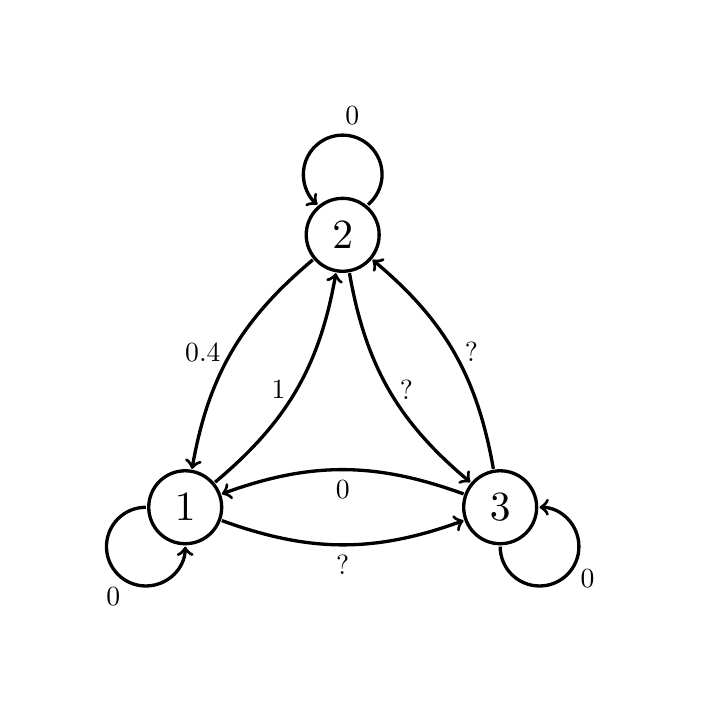
\begin{tikzpicture}
      \node[draw, circle, very thick, scale=1.5] (1) at (0, 0)    {$1$};
      \node[draw, circle, very thick, scale=1.5] (2) at (2, 3.46) {$2$};
      \node[draw, circle, very thick, scale=1.5] (3) at (4, 0)    {$3$};
      \draw[->, very thick]
          (2) edge[bend right=20] node [left]   {$0.4$} (1)
          (1) edge[bend right=20] node [below]  {$?$}   (3)
          (3) edge[bend right=20] node [right]  {$?$}   (2)
          (2) edge[bend right=20] node [right]  {$?$}   (3)
          (1) edge[bend right=20] node [left]   {$1$}   (2)
          (3) edge[bend right=20] node [below]  {$0$}   (1)
          ;
      % self arrows
      % ++(180:5mm) shift the start point to node 2 + (-5mm, 0)
      \draw [->, very thick] (1) ++(180:5mm)
          node [anchor=70, inner sep=10mm] {$0$}
          arc (-270:0:5mm);
      % ++(50:5mm) shift the start point to node 1 + 5mm * (cos(50), sin(50))
      \draw [->, very thick] (2) ++(50:5mm)
          node [anchor=-80, inner sep=10mm] {$0$}
          arc (-50:230:5mm);
      \draw [->, very thick] (3) ++(-90:5mm)
          node [anchor=160, inner sep=10mm] {$0$}
          arc (-180:90:5mm);
    \end{tikzpicture}
  \end{figure}

  \item
  \label{prob1:eigenv}
  Verify that the following three column vectors
  are the right (column) eigenvectors
  of the transition matrix.
  $$
  \mathbf v_1
  =
  \left(
    \begin{array}{r}
      2 \\
      5 \\
      3
    \end{array}
  \right),
  \quad
  \mathbf v_2
  =
  \left(
    \begin{array}{r}
      1 \\
      0 \\
      -1
    \end{array}
  \right),
  \quad
  \mathbf v_2
  =
  \left(
    \begin{array}{r}
      -2 \\
       5 \\
      -3
    \end{array}
  \right),
  $$
  Compute the corresponding eigenvalues.\footnote{
    In this exercise, we are lucky that
    the eigenvectors are known,
    so the eigenvalues can be readily computed
    by the method in the hint.
    %
    Usually, however, we do not know the eigenvectors,
    and then we have to compute the eigenvalues from
    the roots of the cubic equation
    $$
    \det (\mathbf T - \lambda \, \mathbf I) = 0.
    $$
    But if this is too much,
    we have Wolfram Alpha, \url{www.wolframalpha.com}.
    Go there and type something like
    \texttt{
      Eigensystem[\{\{0.4,0.5\},\{0.6,0.5\}\}]}.
  }


  \hint{
    For example, for the last eigenvector,
    we compute the matrix product.
    $$
    \begin{aligned}
    \mathbf T \,
    \mathbf v_3
    &=
    \left(
      \begin{array}{ccc}
        0     & 0.4 &   0 \\
        1     & 0   &   ? \\
        ?     & ?   &   0
      \end{array}
    \right)
    \left(
      \begin{array}{r}
        -2 \\
         5 \\
        -3
      \end{array}
    \right)
    \\
    &
    =
    \left(
      \begin{array}{rrrrrr}
        0 \times (-2) &+& 0.4 \times 5 &+& 0 \times (-3) \\
        1 \times (-2) &+& 0   \times 5 &+& ? \times (-3) \\
        ? \times (-2) &+& ?   \times 5 &+& 0 \times (-3)
      \end{array}
    \right)
    =
    \left(
      \begin{array}{c}
        2 \\
        ?? \\
        ??
      \end{array}
    \right)
    .
    \end{aligned}
    $$
    Hopefully,
    once you have figured out the last two elements,
    you'll find that the result
    is a multiple of $\mathbf v_3$:
    $$
    \mathbf T \,
    \mathbf v_3
    =
    \left(
      \begin{array}{r}
        -2 \, c \\
         5 \, c \\
        -3 \, c
      \end{array}
    \right)
    ,
    $$
    for some value of $c$.
    Then, the value $c$ is the corresponding eigenvalue $\lambda_3$.
  }

  \item
  Identify the eigenvector that corresponds to the eigenvalue $\lambda = 1$.
  Verify that its elements share the same sign.
  Try to normalize it to the stationary distribution, $\mathbf p^s$,
  such that all elements sum to $1.0$.

  \hint{
    Remember that if any vector $\mathbf v$
    is an eigenvector of $\mathbf T$,
    so is any multiple of $\mathbf v$.
    %
    For example, we know
    $\mathbf v_1
    =
    \left(
      \begin{array}{c}
        2  \\
        5   \\
        3
      \end{array}
    \right)
    $
    is a right eigenvector, then
    $10 \, \mathbf v_1
    =
    \left(
      \begin{array}{c}
        20  \\
        50  \\
        30
      \end{array}
    \right)
    $
    is also a right eigenvector.
    %
    Our job is to choose a multiple other than $10$
    such that the elements sum to $1.0$.
    %
    Then the normalized version of $\mathbf v_1$
    can be identified as $\mathbf p^s$.
    %
    Can we also normalize
    $\mathbf v_2$ or $\mathbf v_3$?
    Why or why not?
  }

  \item
  \label{prob1:eigneg1}
  Verify that all eigenvalues satisfy $|\lambda| \le 1$.
  %If there is an eigenvalue with $\lambda = -1$,
  %can we say something about it?

  \item
  Verify that the transition matrix satisfies detailed balance:
  $$
    T_{ij} \, p^s_j = T_{ji} \, p^s_i,
  $$
  for any $i$ and $j$.

  \hint{
    There are only three pairs to verify:
    $(i, j) = (1, 2), (2, 3), (3, 1)$.
    Take the first pair for example,
    we want to verify
    $$
    T_{12} \, p^s_2 = T_{21} \, p^s_1,
    $$
    and we know that $T_{12} = 0.4$
    and $T_{21} = 1$.
  }

  \item
    For each right eigenvector,
    $
    \mathbf v =
    \left(
      \begin{array}{c}
        v_1 \\
        v_2 \\
        v_3
      \end{array}
    \right)
    $,
  compute the corresponding row vector, $\mathbf u$,
  as
  \begin{equation}
    \mathbf u
    =
    \left(
      \frac { v_1 } { p^s_1 }
      , \;
      \frac { v_2 } { p^s_2 }
      , \;
      \frac { v_3 } { p^s_3 }
    \right)
    ,
    \label{eq:ufromv}
  \end{equation}
  verify that every $\mathbf u$
  constructed this way is a left eigenvalue of $\mathbf T$
  with the same eigenvalue.

  \hint{
    To verify a row is a left eigenvector of $\mathbf T$,
    we should see if the matrix product
    $$
    \begin{aligned}
    \mathbf u \, \mathbf T
    &=
    \left(
      u_1, u_2, u_3
    \right)
    \left(
      \begin{array}{ccc}
        0     & 0.4 &   0 \\
        1     & 0   &   ? \\
        ?     & ?   &   0
      \end{array}
    \right)
    \\
    &=
    (u_1 \times 0 + u_2 \times 1 + u_3 \times ?, \\
    &\hphantom{=(}
     u_1 \times 0.4 + u_2 \times 0 + u_3 \times ?, \\
    &\hphantom{=(}
     u_1 \times 0 + u_2 \times ? + u_3 \times 0)
    ,
    \end{aligned}
    $$
    is a multiple of $(u_1, u_2, u_3)$,
    i.e., if it can be written as
    $(c \, u_1, c \, u_2, c \, u_3)$
    for some $c$.
    %
    If so, $\mathbf u$ is an left eigenvector of matrix $\mathbf T$,
    and $c$ is the eigenvalue.
    %
    Now $c$ should match the eigenvalue
    associated with the column vector $\mathbf v$.
    (Is it true for every eigenvector?)

    Here is a mathematical trick to simplify the calculation.
    %
    We know from linearity, that if
    $\mathbf u$ is an eigenvector
    if and only if a nonzero multiple of $\mathbf u$ is
    an eigenvector.
    %
    This means if we get $\mathbf u = (300, 0, -200)$
    from Eq. \eqref{eq:ufromv},
    we can first scale it down to the vector
    $\mathbf u' = (3, 0, -2)$
    and check if $\mathbf u'$ is a left eigenvector.
    %
    This will make the figures smaller, hence more manageable.

    Anyway, the three left eigenvectors, up to multiples, are
    $$
    \begin{aligned}
      \mathbf u_1 &= (1, 1, 1), \\
      \mathbf u_2 &= (3, 0, -2), \\
      \mathbf u_3 &= (-1, 1, -1).
    \end{aligned}
    $$
  }

  \item
  Verify that $\mathbf u_i \cdot \mathbf v_j = 0$
  for any $i \ne j$.

  \hint{
    There are six pairs to check.
    %
    For example, for $i = 2$ and $j = 1$,
    we have
    $\mathbf u_2 = (3, 0, -2)$
    and
    $
    \mathbf v_1 = \left(\begin{array}{r}
        2 \\ 5 \\ 3
    \end{array}\right),
    $
    then
    $\mathbf u_2 \cdot \mathbf v_1
    =
    3 \times 2 + 0 \times 5 + (-2) \times 3
    = 6 + 0 + (-6) = 0.
    $
  }

  \item
  \label{prob1:coarsegraining}
  Construct a coarse-grained transition matrix, $\mathbf S$,
  of two states by merging the first and the third states
  in $\mathbf T$. If we called the merged state $M$, then
  %
  \begin{equation}
  S_{M2} = T_{12} + T_{32},
  \qquad \mathrm{and} \qquad
  S_{2M} =
  \frac{ T_{21} \, p^s_1 + T_{23} \, p^s_3 }
       { p^s_1 + p^s_3 }
  .
  \label{eq:coarse-graining}
  \end{equation}
  %
  Figure out $S_{22}$ and $S_{MM}$
  and complete the transition matrix:
  $$
  \mathbf S
  =
  \left(
    \begin{array}{rr}
      S_{MM}    &   S_{M2} \\
      S_{2M}    &   S_{22}
    \end{array}
  \right).
  $$

%  \item
%  Compute the eigenvalues of $\mathbf S$
%  and compare them with those of $\mathbf T$.
%
%  \item
%  Draw the transition diagram of $\mathbf S$.
%  What can we say about this?
%  Is the process strictly random?
%  Is the Perron-Frobenius theorem still applicable?
%  Reconsider part \ref{prob1:eigneg1}.
%
%  \item
%  Consider the attenuated transition matrix
%  $$
%  \mathbf T'
%  =
%  \frac 1 2
%  \left(
%    \mathbf I
%    +
%    \mathbf T
%  \right)
%  =
%  \left(
%    \begin{array}{ccc}
%      0.5   &   0.2   &   0     \\
%      0.5   &   0.5   &   0.5   \\
%      0     &   0.3   &   0.5
%    \end{array}
%  \right)
%  .
%  $$
%  Show that the eigenvectors of $\mathbf T$
%  are also the eigenvectors of $\mathbf T'$.
%  What are the eigenvalues of $\mathbf T'$?


\end{enumerate}

\end{problem}




\begin{problem}{Coarse-graining}


This is a generalization of the coarse-graining process
in part \ref{prob1:coarsegraining} of the previous problem.
%
In this problem,
we will study how to coarse-graining
an arbitrary transition matrix.

Our strategy is to divide and conquer:
we will break down a complicated process
to a few simple and manageable ones.
%
In this case, we note that every coarse-graining process
can be broken down to a few elementary steps,
such that each elementary step
involves merging only \emph{two} states.

For example, we begin with a system five states,
$1$, $2$, $3$, $4$, and $5$,
and we wish to merge $1$, $2$ and $3$
to state $A$, and merge $4$ and $5$
to state $B$.
%
Then we can break down the task into
three elementary merging steps.
\begin{enumerate}
  \item
    Merge $1$ and $2$ to state $A'$,
    so that we have four states
    $A'$, $3$, $4$ and $5$.

  \item
    Merge $A'$ and $3$ into state $A$,
    so that we have three states
    $A$, $4$ and $5$.

  \item
    Merge $4$ and $5$ into state $B$,
    so that we have
    $A$ and $B$.
\end{enumerate}

What interest us most are the \emph{invariant} properties,
something that never changes before and after
merging two states.
%
Now the nice thing is that if an invariant property
holds before and after any elementary step,
then it holds before and after the entire
process.\footnote{For example,
  the total energy is an invariant quantity
  for the molecular dynamics (MD) simulation.
  The total energy should be the same before and after
  each MD step. So can we assert that the total
  energy at the beginning of an MD simulation
  is the same as the total energy at the end
  of the simulation.
}

Below, we wish to show that the basic properties
of the transition matrix are invariant properties.
%
Besides, detailed balance is also an invariant.



%
%\footnote{In
%  computer science,
%  many elegant algorithms involving loops,
%  such as binary search, quick sort, etc,
%  have loop invariants:
%  some thing that does not change
%  after the execution of each loop.
%  %
%  In understanding and implementing these algorithms,
%  it is critical to check if the loop invariance
%  holds.
%}
%


\begin{enumerate}
  \item
  Convince yourself that any coarse-graining process
  can be broken down to a sequence
  of two-state-merging processes.

  \item
  Generalize
  Eq. \eqref{eq:coarse-graining}
  for the two-state-merging process.
  %
  Note that there might be more than one
  remaining states.
  %
  How do they affect
  Eq. \eqref{eq:coarse-graining}?
  %
  For simplicity, we may assume that
  the two to-be-merged states are $1$ and $2$,
  and the remaining states are $j = 3, 4, \dots$.

  \item
  Show that the coarse-grained matrix satisfies
  the three basic rules of a transition matrix:
  (i) $S_{ij} \ge 0$,
  (ii) $\sum_i S_{ij} = 1$,
  (iii) $\sum_j S_{ij} \, P^s_j = P^s_i$.
  Here, $\mathbf P^s$ is the distribution
  \emph{after} the two-state-merging.

  \item
  If the original transition matrix satisfies detailed balance,
  show that the transition matrix after the two-state-merging
  also satisfies detailed balance.
\end{enumerate}

\end{problem}





\section{Answer keys}


\begin{problem}{Getting familiar with transition matrices}
\begin{enumerate}
  \item
  $$
    \mathbf T
    =
    \left(
      \begin{array}{ccc}
      0       &   0.4   &   0  \\
      1       &   0     &   1  \\
      0       &   0.6   &   0
      \end{array}
    \right)
    .
  $$

  \item
  See the diagram below.
  \begin{figure}[h]
    \centering
    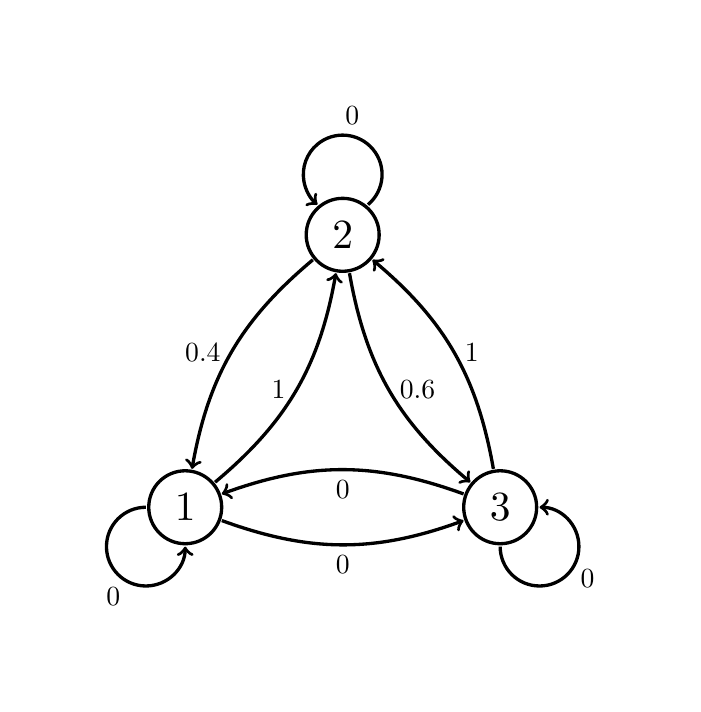
\begin{tikzpicture}
      \node[draw, circle, very thick, scale=1.5] (1) at (0, 0)    {$1$};
      \node[draw, circle, very thick, scale=1.5] (2) at (2, 3.46) {$2$};
      \node[draw, circle, very thick, scale=1.5] (3) at (4, 0)    {$3$};
      \draw[->, very thick]
          (2) edge[bend right=20] node [left]   {$0.4$} (1)
          (1) edge[bend right=20] node [below]  {$0$}   (3)
          (3) edge[bend right=20] node [right]  {$1$}   (2)
          (2) edge[bend right=20] node [right]  {$0.6$} (3)
          (1) edge[bend right=20] node [left]   {$1$}   (2)
          (3) edge[bend right=20] node [below]  {$0$}   (1)
          ;
      % self arrows
      % ++(180:5mm) shift the start point to node 2 + (-5mm, 0)
      \draw [->, very thick] (1) ++(180:5mm)
          node [anchor=70, inner sep=10mm] {$0$}
          arc (-270:0:5mm);
      % ++(50:5mm) shift the start point to node 1 + 5mm * (cos(50), sin(50))
      \draw [->, very thick] (2) ++(50:5mm)
          node [anchor=-80, inner sep=10mm] {$0$}
          arc (-50:230:5mm);
      \draw [->, very thick] (3) ++(-90:5mm)
          node [anchor=160, inner sep=10mm] {$0$}
          arc (-180:90:5mm);
    \end{tikzpicture}
  \end{figure}

  \item
    $
      \lambda_1
      =
      1,
      \mathbf v_1
      =
      \left(
        \begin{array}{r}
          2 \\
          5 \\
          3
        \end{array}
      \right)
      ,
      \lambda_2
      =
      0,
      \mathbf v_2
      =
      \left(
        \begin{array}{r}
          1 \\
          0 \\
          -1
        \end{array}
      \right)
      ,
      \lambda_3
      =
      -1,
      \mathbf v_3
      =
      \left(
        \begin{array}{r}
          -2 \\
          5 \\
          -3
        \end{array}
      \right)
      .
    $

    To figure out the eigenvalues directly:
    $$
    \begin{aligned}
    0
    &=
    \left|
      \begin{array}{ccc}
      -\lambda  &   0.4   &   0  \\
      1         & -\lambda  &   1  \\
      0         &   0.6   &   -\lambda
      \end{array}
    \right|
    =
    -\lambda \, (\lambda^2 - 0.6) + 0.4 \, \lambda
    =
    \lambda - \lambda^3
    .
    \end{aligned}
    $$
    So $\lambda = 0$ or $\pm 1$.

  \item
    The eigenvector is $\mathbf v_1$,
    $
      \mathbf p^s
      =
      \frac{1}{10} \mathbf v_1
      =
      \left(
        \begin{array}{r}
          0.2 \\
          0.5 \\
          0.3
        \end{array}
      \right)
      .
    $

  \item
    $|1| \le 1$, $|0| \le 1$, and $|-1| \le 1$.

  \item
    For $1$ and $2$, $1 \times 0.2 = 0.4 \times 0.5$;
    for $2$ and $3$, $0.6 \times 0.5 = 1 \times 0.3$;
    for $1$ and $3$, $0 \times 0.2 = 0 \times 0.3$.

  \item
    $$
    \begin{aligned}
      \mathbf u_1 &= (1, 1, 1),
      &
      \mathbf u_1 \, \mathbf T &= (1, 1, 1)
      , \\
      \mathbf u_2 &= (3, 0, -2),
      &
      \mathbf u_2 \, \mathbf T &= (0, 0, 0)
      , \\
      \mathbf u_3 &= (-1, 1, -1),
      &
      \mathbf u_3 \, \mathbf T &= (1, -1, 1)
      .
    \end{aligned}
    $$
\end{enumerate}
\end{problem}


\end{document}
